%%%%%%%%%%%%%%%%%%%%%%%%%%%%%%%%%%%%%%%%%%%%%%%%%%%%%%%%%%%%%%%%%%%%%%%%%%%%%%%%
%2345678901234567890123456789012345678901234567890123456789012345678901234567890
%        1         2         3         4         5         6         7         8

\documentclass[letterpaper, 10 pt, conference]{ieeeconf}  % Comment this line out
                                                          % if you need a4paper
%\documentclass[a4paper, 10pt, conference]{ieeeconf}      % Use this line for a4
                                                          % paper

\IEEEoverridecommandlockouts                              % This command is only
                                                          % needed if you want to
                                                          % use the \thanks command
\overrideIEEEmargins
% See the \addtolength command later in the file to balance the column lengths
% on the last page of the document



% The following packages can be found on http:\\www.ctan.org
\usepackage[utf8x]{inputenc} %for linux 
%\usepackage[UTF8]{inputenc} %for windows
\usepackage{graphics} % for pdf, bitmapped graphics files
%\usepackage{epsfig} % for postscript graphics files
\usepackage{graphicx}
\usepackage{mathptmx} % assumes new font selection scheme installed
%\usepackage{times} % assumes new font selection scheme installed
\usepackage{amsmath} % assumes amsmath package installed
\usepackage{amssymb}  % assumes amsmath package installed

\usepackage{algorithm}
%\usepackage[options]{algorithm2e}
\usepackage[linesnumbered,lined,boxed,commentsnumbered,ruled]{algorithm2e}
\usepackage[noend]{algpseudocode}
\usepackage{float}
\usepackage{cases}
\usepackage{xcolor}
\usepackage{bm}

% If your conference documentclass or package defines these macros,
% change these macros to different names.
\newcommand*{\affaddr}[1]{#1} % No op here. Customize it for different styles.
\newcommand*{\affmark}[1][*]{\textsuperscript{#1}}
\newcommand*{\email}[1]{\texttt{#1}}

\bibliographystyle{plain}  

\title{\LARGE \bf
Learning pose constraints for trajectory optimization from demonstration}

\author{% 
Dominique M. Tao\affmark[1], Baris Akgun\affmark[2], Andrea L. Thomaz\affmark[2] and Aude Billard\affmark[1]\\\\
\parbox{3 in}{\centering \affaddr{\affmark[1]Learning Algorithms and Systems Laboratory\\
\affaddr{EPFL, Switzerland}\\
\email{\{dominique.tao,aude.billard\}@epfl.ch}\\
}}
\hspace*{ 0.7 in}
\parbox{3 in}{\centering \affaddr{\affmark[2]Socially Intelligent Machine Lab\\
Department of Computer Science \\
\affaddr{UT Austin, USA }\\
\email{barisakgun@gmail.com\\
athomaz@ece.utexas.edu}\\ 
}}}
\newcommand{\trsp}{{\!\scriptscriptstyle\top}}
\newcommand{\mb}[1]{{\boldsymbol{#1}}}
\newcommand{\psin}{{\!\dagger}}
\newcommand\norm[1]{\left\lVert#1\right\rVert}
\newcommand{\dosemic}{\renewcommand{\@endalgocfline}{\algocf@endline}}% Reinstate semi-colon ;
\newcommand{\pushline}{\Indp}% Indent
%\author{
%\parbox{3 in}{\centering Huibert Kwakernaak*
%         \thanks{*Use the $\backslash$thanks command to put information here}\\
%         Faculty of Electrical Engineering, Mathematics and Computer Science\\
%         University of Twente\\
%         7500 AE Enschede, The Netherlands\\
%         {\tt\small h.kwakernaak@autsubmit.com}}
%         \hspace*{ 0.5 in}
%         \parbox{3 in}{ \centering Pradeep Misra**
%         \thanks{**The footnote marks may be inserted manually}\\
%        Department of Electrical Engineering \\
%         Wright State University\\
%         Dayton, OH 45435, USA\\
%         {\tt\small pmisra@cs.wright.edu}}
%}

%\author{Dominique Tao, Baris Akgun, Andrea L. Thomaz and Aude Billard}% <-this % stops a space

%\thanks{This work was not supported by any organization}% <-this % stops a space
%\thanks{H. Kwakernaak is with Faculty of Electrical Engineering, Mathematics and Computer Science,
%        University of Twente, 7500 AE Enschede, The Netherlands
%        {\tt\small h.kwakernaak@autsubmit.com}}%
%\thanks{P. Misra is with the Department of Electrical Engineering, Wright State University,
%        Dayton, OH 45435, USA
%        {\tt\small pmisra@cs.wright.edu}}%
%}

\makeatletter
\newcommand{\removelatexerror}{\let\@latex@error\@gobble}
\makeatother

\begin{document}

\maketitle
\thispagestyle{empty}
\pagestyle{empty}


%%%%%%%%%%%%%%%%%%%%%%%%%%%%%%%%%%%%%%%%%%%%%%%%%%%%%%%%%%%%%%%%%%%%%%%%%%%%%%%%
\begin{abstract} 
When performing a task in presence of obstacles, there are multiple directions the manipulator could take to avoid them and still successfully execute the task. 
In the context of Keyframe-based Learning from Demonstration applied to robot manipulator, we present a framework with a sampling-based planner that
  generates a trajectory based on the intention of the user which indicates towards which direction the robot should first try to move in order to avoid obstacles while executing the task.
 Our approach first constructs a geometric constraint of the space between two Gaussians of the model, that we call Soft-Envelope, to constrain the movement of the robot. Dimension reduction is used on the Soft-Envelope to extract important aspects from the learned skill. Then we used our RRT* sampling-based motion planner to generate a trajectory  w.r.t to the Soft-Envelope. It uses a double sampling approach combined with a natural gradient descent projection and Jacobian transform in order explore the C-space while being constrained around the Soft-Envelope. The tree is grown in C-space by only using samples inside a C-space subset corresponding to the Soft-Envelope in workspace. \\
Kinesthetic teachning is used to collect keyframes data from a real 6-DOF Kinova Jaco arm. Our algorithm is then tested with the same robot in simulation. During the execution, new unseen obstacles are introduced to hinder the movement.
\end{abstract}

\begin{keywords}
Keyframe-based Learning from Demonstration approach (KLfD), sampling-based motion planning, geometric constraints (Soft-Envelope), dimension reduction, natural gradient descent projection.
\end{keywords}
%%%%%%%%%%%%%%%%%%%%%%%%%%%%%%%%%%%%%%%%%%%%%%%%%%%%%%%%%%%%%%%%%%%%%%%%%%%%%%%%

\section{INTRODUCTION}
Kinesthetic teaching in a Learning from Demonstration context is a widely used approach that allows an user to easily provide demonstrations to the robot by physically guiding it when performing a skill as shown in figure \ref{Pic_kinesthetik_teaching}. However, when executing the learned skill from demonstrations, the robot may encounter new and unseen obstacles that were not present during teaching while executing the skill. Different actions and directions can be undertook by the robot to avoid them  and still complete the task.\\
If we take the pouring water skill illustrated in figure \ref{Pic_kinesthetik_teaching} as an example and we insert an obstacle mid-way, one possible action is to have the user re-demonstrate the skill to take them into account, and thus indicating one possible direction among many possible others to avoid the obstacle. It is often the case when using a regression technique (GMM-GMR) \cite{SylvainLearningGeneralizing} \cite{Calinon15} or spline interpolation \cite{refKeyframe1} to create the skill, the obstacle has to be present in both teaching and execution or new demonstrations need to be provided to take them into account. Still in the context of regression technique, reinforcement learning is an action that can be undertaken to enable the learning of new solution without the intervention of the user\cite{ReinforcementLearningAude}. 
An other course of action is to use a motion planner such as a potential field \cite{PotentialField} or a sampling based-planner(RRT \cite{RRTandLFD}, PRM\cite{ModelAndPRM}), combined with the learned model, to create an end-to-end trajectory for the execution of the task without the intervention of the user, but the obstacle avoidance is done more randomly. Although these methods successfully accomplish the task, they only select one or random directions for the robot to avoid an obstacle and sometimes require the intervention of the user.\\

\begin{figure}[ht]
	\centering
	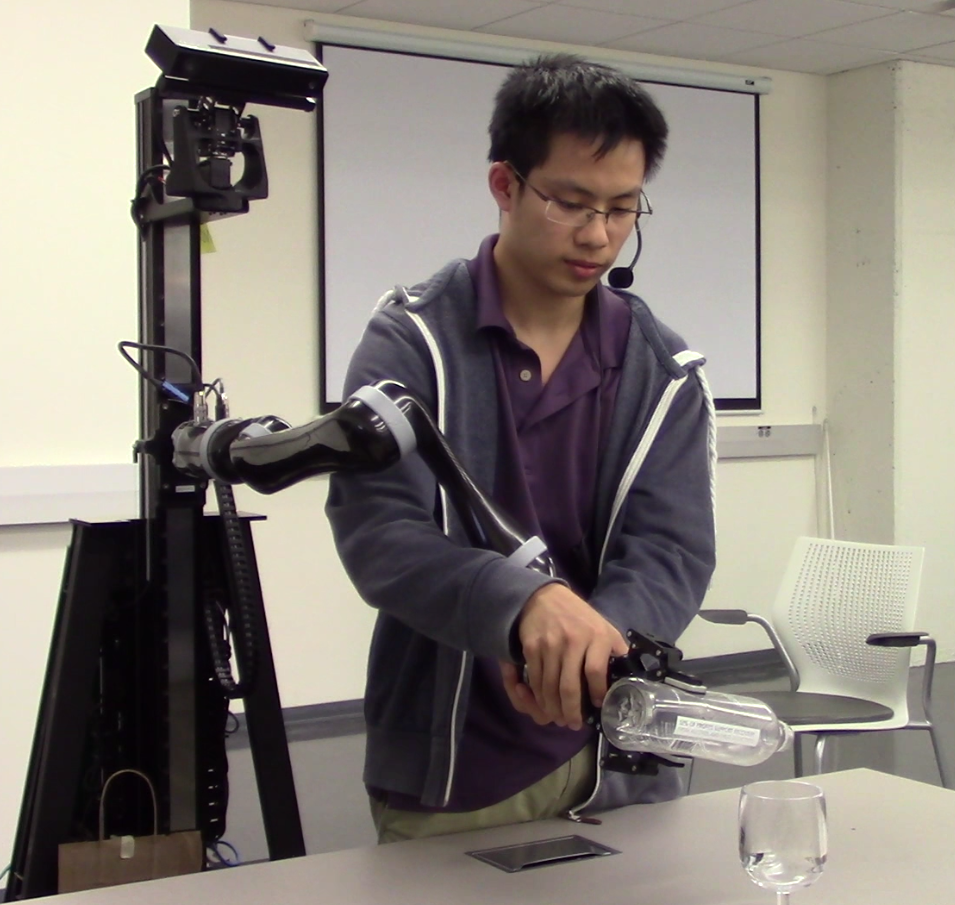
\includegraphics[scale=0.2]{figure/kinesthetic_teaching.png}
	\caption{A teacher using kinesthetic teaching with a 6-DOF Kinova Jaco arm to demonstrate a pouring water skill}
	\label{Pic_kinesthetik_teaching}
\end{figure}

Our objective in this framework is then two-fold: 1) to enable the robot to avoid, without the help of the user, new static obstacles during its execution  2) indicate to the robot a first direction (which we assimilate as the user intention when he demonstrated the skill to the robot) to try in order to avoid obstacles before it tries other directions.\\

In this paper, we use keyframes demonstration provided by kinesthetic teaching to learn the skill. Keyframes are a sparse set of sequential points or critical points in space. They are also referred as \textit{via-points} in industrial robot programming. During the demonstrations, the user moves the robot to the desired pose and records a keyframes. The resulting skill model is composed of multivariate Gaussians that are clustering these keyframes.\\
We also made the assumption that the biggest variance of each Gaussian of the model reflects the intention of the user when demonstrating the skill. This variance is identified as the first direction that the robot should try to move to avoid an obstacle. For instance, with the pouring water skill, we expect the demonstration of the Gaussian above the glass to have more variance in its vertical direction since there is less restriction from where the water is spill. 
 
 \subsection{Proposed Approach}
To satisfy the above-mentioned objectives, we combine the learned skill model which specify constraints in space (position and orientation for the end-effector to perform the task) with the performance of a RRT* sampling-based planner, introduced by Karaman \cite{KaramanRRTStar}.\\
Our motivation to use such an planner lies in its abilities to efficiently find a feasible and collision-free path that randomly explore any direction by growing a tree in space with an iterative sampling and without the user intervention. Furthermore, RRT* is probabilistically complete and asymptotically optimal if the sampling (done uniformly) and the growth of the tree are in the configuration space (C-space) of the robot, meaning that the planner is guaranteed to find a solution, if it exists, and that is optimal as the number of samples approaches infinity.\\
The planner that we proposed in this work is an extension of a RRT* that was designed to efficiently sample inside a constrained manifold. In fact, while the keyframes clusters are efficient to encapsulate the essence of the skill, there is no information on how the motion should be executed between two clusters, as they are sparsely distributed in space. To solve this issue and also for the used of our planner, we constructed a constrained area between two considered Gaussians, that we named "Soft-Envelope".\\
In order to influence the motion w.r.t the intention of the user, dimension reduction method is applied on the Soft-Envelope, resulting in a "Reduced Soft-Envelope". If correctly reduced, it enables our planner to direct its trajectory along the some principal directions by constraining its sampling inside the reduced region that reflects  the biggest variance along the Soft-Envelope.\\
Even though there is no proof of it in this paper, we are still interested in satisfying the criteria of completeness and optimality for RRT* as just mentioned above. Hence our planner uses a double sampling process in order to uniformly explore the C-space while trying to have its tree growing inside the Soft-Envelope. Natural gradient descent projection and Jacobian transform are also used for this reason.\\
Moreover, the Jacobian transform is used instead of an IK solver to find the joint configuration, allowing our algorithm to be generalized for manipulator with more than 6 DOF where the IK solver might have  encountered problems with infinite solutions for a given pose.

\subsection{Related Works}
 Berenson \textit{et al.} have done many works in sampling-based planning and constrained manifold that can relate to ours. He introduces the concept of Workspace Goal Region \cite{Berenson_WGR} or Task Space Regions(Chains) \cite{BerensonTSR} which is a 6-dimensional volume in workspace specifying the goal sets for their planner. Although these constraints are intuitive to specify, can efficiently be sampled and the distance from a joint configuration to one of this constraint can be easily calculated, they need to be manually set depending on the task. In our work, the multivariate Gaussians from the skill model can be assimilated to the Task Space Regions, sharing all their advantages, but is instead automatically defined by the user when he provided the demonstration. Our Soft-Envelope constraints can be assimilated to the concept of Task Space Region Chains but also do not need to be manually defined as it follows naturally from the Gaussian clusters of the skill model.
In addition, a similar representation of our Soft-Envelope constraint can be found in \cite{CanalSpace} with the Canal Space proposed by Ahmadzadeh \textit{et al.}  who uses it to encode demonstrations in order to learn a skill model.\\
Berenson \textit{et al.} also work on a planners using projection technique \cite{Berenson_WGR} \cite{Berenson_Gradient} by projecting the joint configuration onto their constrained manifold (proof of completeness is done in \cite{Berenson_2010_6558} ). Similarly, our planner also use projection technique with a gradient descent but instead project one pose in workspace onto another one inside the Soft-Envelope because it is more easy to express the distance w.r.t to a gaussian in workspace. The projection is used as a feed-forward to guide the joint configuration inside a subspace of C-space corresponding to the Soft-Envelope in Workspace. \\

Another body of work have been done combining PCA dimension reduction method with a sampling-based planner to bias the RRT planner toward directions which it would not normally explore \cite{balancing_statespace_coveragePCA} or to favor the direction along which the roadmap tree is high \cite{PCARRT2}. PCA is also used with PRM planner to influence the sampling into difficult regions with low clearance in C-space \cite{PCA_PRM}. In our work, we use eigenvalues/vectors-decomposition to influence sampling and the growth of the tree along the principal component of each Gaussian used to create our constrained region in workspace.\\

\section{Method}
After collecting keyframes data (joint configuration and its corresponding pose) from kinesthetic teaching, the model is learned by using a HMM which gives as an output an ordered sequence of multivariate Gaussians in workspace to reproduce the skill. A more detailed explanation of the procedure is given in \cite{KeyframesSelfLearning}.
 At each time, our method is used on only two connected Gaussians from the given states sequence to construct a local trajectory, going respectively from what we called the "parent" to the "child" Gaussian. The full trajectory used to recreate the task can easily be generated by combining all the local trajectories together.
The different parts of the algorithm are summarized in the pseudo-code of algorithm \ref{planning}. \\

Let $\mb{q} \in \mathbb{R}^{M \times 1}$ a joint configuration in C-Space of dimension $M$  and $\mb{p} \in \mathbb{R}^{N \times 1}$ a pose in workspace of dimension $N$. $\mb{\Sigma}_{p} , \mb{\Sigma}_{c} \in \mathbb{R}^{N \times N}$  and $\mb{\mu}_{p} , \mb{\mu}_{c} \in \mathbb{R}^{N \times 1}$ are respectively the covariance and center of the parent and child gaussians.
The parameter $\alpha$ is used as the percentage of the data to be represented in the dimension reduction technique. The joint vector $\mb{q}_{start}$, with $\mb{p}_{start}$ its corresponding pose in workspace, is either the initial configuration of the robot or the last joint of the local trajectory solution from the previous pair of gaussians. \\

\begin{algorithm}[H]
 \caption{Planning($\mb{\Sigma}_p,\mb{\mu}_p,\mb{\Sigma}_c,\mb{\mu}_c,\alpha$)}\label{planning}

\SetKwData{Left}{left}\SetKwData{This}{this}\SetKwData{Up}{up}
\SetKwFunction{Union}{Union}\SetKwFunction{FindCompress}{FindCompress}
\SetKwInOut{Input}{input}\SetKwInOut{Output}{output}
\Output{Local trajectory from parent to children gaussian}
\BlankLine
\setcounter{AlgoLine}{0}
$[Q_q,Q_p] \leftarrow \mb{q}_{start},\mb{p}_{start}$;

$E \leftarrow \emptyset$;

$X_{sol} \leftarrow \emptyset$;

$G=(Q_q,Q_p,E,Q_{sol})$;
\BlankLine
$[\mb{\Sigma}_{envSet},\mb{\mu}_{envSet}] \leftarrow$ Soft\_Envelope($\mb{\Sigma}_p,\mb{\mu}_p,\mb{\Sigma}_c,\mb{\mu}_c$);

$\mb{\Sigma}_{redEnvSet} \leftarrow$ Reduced\_Soft\_Envelope($\mb{\Sigma}_{envSet}$,$\mb{\Sigma}_{p}$,$\mb{\Sigma}_{c}$, $\alpha$);

\BlankLine
PCTC\_RRTStar($G$,$\mb{\Sigma_{envSet}}$,$\mb{\Sigma_{redEnvSet}}$,$\mb{\mu_{envSet}}$, $\alpha$);

\end{algorithm}
For our variation of the RRT* algorithm, we initialize the tree with  $T=(Q,E,Q_{sol})$ with $Q \subset Q_{free}$ the set of all vertices in C-space, the edges $E \subset Q_{free} \times Q_{free}$ and $Q_{sol}$ the set of joints configuration inside the child gaussian, used to indicate that a path is found. The set $Q$ is a double set $Q_q$ and $Q_p$ which respectively store the joint configuration used to grow the tree in C-space and also its corresponding pose in workspace. 

\subsection{Calibration}
\subsubsection{Child and Parent Gaussian}\leavevmode\par
For a given initial pose $\mb{p}_{init}$ of the end-effector, the first step is to know which pair of connected Gaussians to consider as parent and child for our planner.\\
We calculate the euclidean distance from $\mb{p}_{init}$ to each Gaussians center of the given state sequence and then select the Gaussian $G^s$ that gives the minimal distance.
Since $G^{s}$ is from a sequence of ordered Gaussians, it is at most connected to a previous $G^{s-1}$ and next Gaussian $G^{s+1}$.  The euclidean distances from the pose $p_{init}$ to the center of $G^{s-1}$ and $G^{s+1}$, $\norm{\overrightarrow{\mb{p_{init}}\mb{\mu^{s-1}}}}$ and $\norm{\overrightarrow{\mb{p_{init}}\mb{\mu^{s+1}}}}$, are then calculated and compared to see which gaussian is to be paired with $G^s$ for the first used of algorithm \ref{planning}.\\
If $\norm{\overrightarrow{\mb{p_{init}}\mb{\mu^{s-1}}}}$ is smaller, then $G^{s-1}$ becomes the parent and $G^{s}$ the child Gaussian (the same logic with  $G^{s}$ becoming the parent and $G^{s+1}$ the child Gaussian if $\norm{\overrightarrow{\mb{p_{init}}\mb{\mu^{s+1}}}}$ was smaller).\\

\subsubsection{Soft-Envelope}\leavevmode\par
We introduce a constrained area between two considered Gaussians  of the model with the intention of having a constrained region inside which we would like the motion of the end-effector to be, which is why we called it "Soft-Envelope". An illustration is shown in figure \ref{MixSoftEnvelope}.\\ 
\begin{figure}[h]
	\centering
	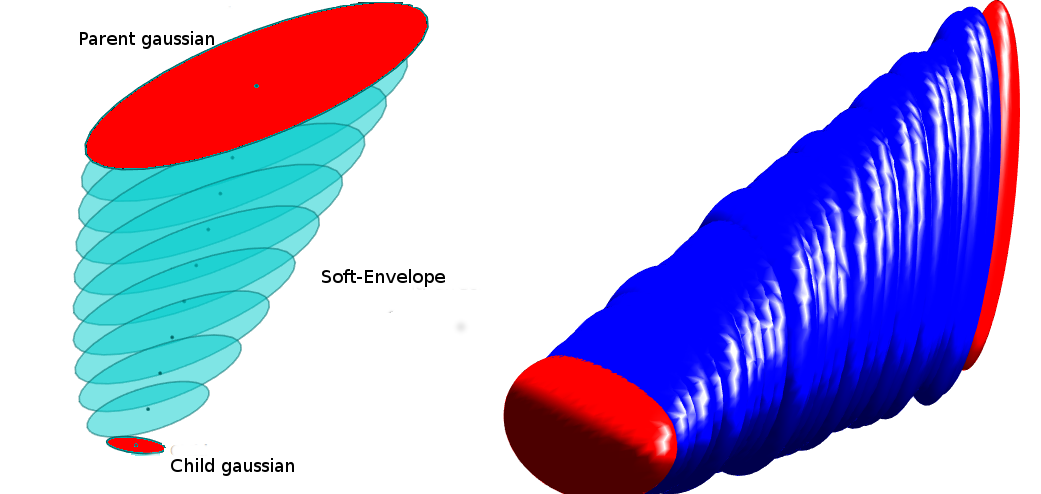
\includegraphics[scale=0.23]{figure/MixSoftEnvelope.png}
	\caption{Representation of the Soft-Envelope in 2D and 3D ($\mathbb{R}^{3}$)}
	\label{MixSoftEnvelope}
\end{figure}
\\
 In fact, in a keyframe-based learning from demonstration, the skill is only encoded by a sparse set of keyframes Gaussians in workspace and hence there is no telling how the end-effector should move between two clusters of the model (parent and child), especially when using a sampling-based motion planner which constructs a trajectory by sampling the space.\\
 It is also used as a sampling region to guide the creation of the trajectory. Only sampling inside the "child" Gaussian, depending on its size, may not be enough to efficiently grow an end-to-end path in presence of obstacles and sampling in the full C-space of the arm may lead the trajectory away from the goal, with the consequences of waiting a long time before convergence.\\
 
The Soft-Envelope is created by linear interpolation of the parent/child covariance matrices and centers as shown in the following equations: 
\begin{subnumcases}{}
			 \mb{\mu_{env}}^{0}= \mb{\mu_{p}}  \\
			 \mb{\Sigma_{env}}^{0}=\mb{\Sigma_{p}}\\
			 \mb{\mu_{env}}^{i+1} = \mb{\mu_{env}}^{i}+(\mb{\mu_{c}}-\mb{\mu_{p}})\triangle d \\
			 \mb{\Sigma_{env}}^{i+1} = \mb{\Sigma_{env}}^{i}+(\mb{\Sigma_{c}}-\mb{\Sigma_{p}})\triangle d 
			 \label{equaInterCov}
\end{subnumcases}
with $\mb{\mu_{env}}^i \in \mathbb{R}^{N \times 1}$ and $\mb{\Sigma_{env}}^i \in \mathbb{R}^{N \times N}$ the center and covariance matrix of the $i^{th}$ gaussian of the Soft-Envelope. We define $\mb{\Sigma_{envSet}}$ the set of all the calculated matrices $\mb{\Sigma_{env}}$ forming the Soft-Envelope and $\mb{\mu_{envSet}}$ the set of all $\mb{\mu_{env}}^i$ .\\ 
 Though the coefficient $\triangle d $ can be chosen as a result of a function with respect to the euclidean distance of the two center ${\norm{\overrightarrow{\mb{\mu}_p\mb{\mu}_c}}}$ , we decided instead to use a small number (w.r.t. the biggest and smallest distance between two linked gaussians in the model) since not all pair of gaussians in the model are evenly separated.\\
Furthermore, the Soft-Envelope can automatically be adapted to any pair of Gaussians and has the advantage of being easily sampled in a uniform way since it is only composed of a series of Gaussians (see section \ref{samplingSection}).\\

\subsubsection{Reduced Soft-Envelope}\leavevmode\par \label{ReducedSoftEnvelope}
As the variance of a Gaussian in the model can be interpreted as the intention of the user when the skill was demonstrated, the Gaussians of the Soft-Envelope are then viewed as a linear transition of the user intention. They are hence used as a way to influence (indicate to) the end-effector which directions it should first try to move, when going from the parent to the child Gaussian, in order avoid obstacles. \\
The idea to do so is to encapsulate the direction with the biggest variances in each of its Gaussians by using an eigenvalues/vectors decomposition technique, creating  a "Reduced-Soft-Envelope" in full workspace that we used, instead of the Soft-Envelope, for the sampling and for the evaluation of any point belongings to it.
The process is illustrated in algorithm \ref{AlgoRedSoftEnve}.\\

As a fact, one has first to remember that only the parent and the child Gaussians of the model truly represent the variance allowed for the task, the Soft-Envelope being just one linear interpretation of how the variances should evolve between these two. Hence, our first step uses eigenvalues decomposition separately on the child and parent Gaussians to determine the number of eigenvector needed to represent $\alpha \%$ of the data, with $\alpha$ a parameter specified by the user. We compare them and take the biggest number of eigenvector as $N_{eig}$ (line 2-5). \\
 Each of the Soft-Envelope Gaussians covariance matrix $\mb{\Sigma}_{env}^i \in \mathbb{R}^{N \times N}$  are then decomposed into a full eigenvector matrix $\mb{V}^{i} \in \mathbb{R}^{N \times N}$ and diagonal eigenvalue matrix $\mb{D}^{i} \in \mathbb{R}^{N \times N}$. The reduced  matrix $\mb{V}_{red}^{i}\in \mathbb{R}^{N \times N_{eig}}$ and $\mb{D}_{red}^{i} \in \mathbb{R}^{N_{eig} \times N_{eig}}$ are created by using the $N_{eig}$ biggest eigenvectors and associated eigenvalues.\\
The full reduced covariance matrix from $\mb{\Sigma}_{env}^{i}$ is finally calculated with $\mb{\Sigma}_{red}^{i} =\mb{V}_{red}^{i} \mb{D}_{red}^{i}  (\mb{V}_{red}^{i})^{\psin}$, such that $\mb{\Sigma}_{red}^{i}  \in \mathbb{R}^{N \times N} $  is the covariance matrix of the $i^{th}$ Gaussian of the reduced Soft-Envelope (line 8-10). Each of this new covariance matrix belongs to the set $\mb{\Sigma}_{redEnvSet}$. A visual representation is shown in figure \ref{100vs90EnvOnly}.
\begin{algorithm}[H]
 \caption{Reduced\_Soft\_Envelope($\mb{\Sigma_{envSet}}$,$\mb{\Sigma_{p}}$,$\mb{\Sigma_{c}}$, $\alpha$)}\label{AlgoRedSoftEnve}

\SetKwData{Left}{left}\SetKwData{This}{this}\SetKwData{Up}{up}
\SetKwFunction{Union}{Union}\SetKwFunction{FindCompress}{FindCompress}
\SetKwInOut{Input}{input}\SetKwInOut{Output}{output}
\Output{All $\mb{\Sigma_{red}}^i$ of the Reduced Soft-Envelope ($\Sigma_{redEnvSet}$ the set of all $\mb{\Sigma_{red}}^i$)}
\BlankLine
 \setcounter{AlgoLine}{0}

\emph{//Number of eigenvector $N_{eig}$ to represent $\alpha\%$ of the data}\;

$N_{eigP}$ $\leftarrow$ Extract\_N\_EigenDecomp($\mb{\Sigma_{p}}$, $\alpha$);\;

$N_{eigC}$ $\leftarrow$ Extract\_N\_EigenDecomp($\mb{\Sigma_{c}}$, $\alpha$);\;

\lIf{ $N_{eigC}$ $<$ $N_{eigP}$}{$N_{eig} = N_{eigP}$}\lElse{$N_{eig} = N_{eigC}$}{}
\BlankLine

\emph{//Reduced Soft-Envelope}\;


\For{$i\leftarrow $ 1 \KwTo size($\mb{\Sigma_{envSet}}$)}
{ 
	$[\mb{V}^i,\mb{D}^i] \leftarrow$ Eigen\_Decomp($\mb{\Sigma_{env}}^i$); \;
	
	$[\mb{V}_{red}^{i},\mb{D}_{red}^{i}] \leftarrow$ Reduce\_Mat($\mb{V}^i,\mb{D}^i,N_{eig}$);\;
	
	 $\mb{\Sigma_{red}}^{i} =\mb{V}_{red}^{i} \mb{D}_{red}^{i}  (\mb{V}_{red}^{i})^{\psin}$;\;
	\BlankLine
	\emph{//Calculate nearest positive definite matrix (Higmam method) and regularization }\;
	
	$\mb{\Sigma_{red}}^{i} \leftarrow$  Nearest\_PDMat($\mb{\Sigma_{red}}^{i}$);\;
	\BlankLine
	$EigVal_{Smallest} \leftarrow$ Eigen\_Decomp($\mb{\Sigma_{red}}^{i}$);\; 
	
	k=0 and $\epsilon= FLT\_EPSILON $;
	
	\While{$EigVal_{Smallest}<0$}{
	
		k++;
		
		$\mb{\Sigma_{red}}^{i}$=	$\mb{\Sigma_{red}}^{i} + (-EigVal_{Smallest} \times k^2 + \epsilon) \times \bf{I}$;
	}
}
\end{algorithm}


\begin{figure}[h]
	\centering
	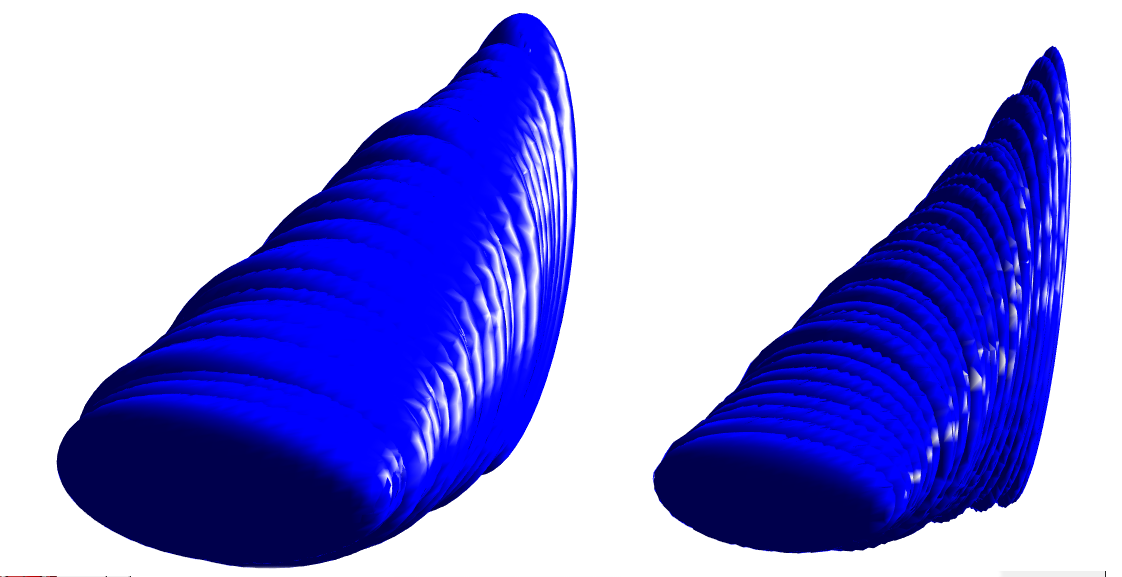
\includegraphics[scale=0.35]{figure/100vs90EnvOnly.png}
		\caption{Representation in ($\mathbb{R}^{3}$) of the same Soft-Envelope (left image)without dimension reduction ($\alpha = 100 \%$) and (right image) with dimension reduction($\alpha = 90\%$ reduced Soft-Envelope); We can see the effect of the reduction that redefined the contour and make the Gaussian smaller w.r.t the selected eigenvectors.}
	\label{100vs90EnvOnly}
\end{figure}

One particular aspect to be cautious with the reduced Soft-Envelope is to make sure that its Gaussians are still semi-positive definite because they will be used later to calculate a quadratic distance (Mahalanobis distance). In fact, $\mb{\Sigma}_{red}^{i}$ being calculated by approximation of eigenvectors and eigenvalues matrices can have approximation of very small values making it just not positive definite.\\ One way to correct this problem is to use the method introduced by Higham in \cite{Nearest_PSDMATRIX} to calculate the nearest symmetric semi-definite positive matrix that we combine with a regularization process using the smallest eigenvalue until the matrix is positive definite (line 12-18).

\subsection{PCT-RRT*} \label{PCT-RRT*}
Our sampling-based planner (Projection Constrained Taskspace -RRT*) PCT-RRT* is an extension of the RRT*: the work has been more focus on how the sampling should be considered to grow a single tree in C-space while being influenced by the Soft-Envelope, however the core of the planner remains a RRT*. The pseudo-code of the procedure is presented in the algorithm \ref{PCTCRRT}.\\
As our interest lies in growing the tree inside the Soft-Envelope while being able to explore the C-space (one of the necessary condition for the completeness of the planner), we use, at each iteration, a double sampling process (line 3,7,8). \\

At each iteration, a first sample, $\mb{p}_{sRef}$, is created inside the Soft-Envelope in workspace and its joint configuration is used to grow the tree in C-space. To generate its IK solution, we use a second sampling, $\mb{q}_s$, in the full C-space, and iteratively project, in a second intern loop, its corresponding pose $\bm{p}_s^j$ onto  $\mb{p}_{sRef}$ by using a gradient descent process combined with the Jacobian transform.\\
During the projection process (line 10-33), the natural gradient descent is used to iteratively calculate the next pose $\mb{p}_s^{j+1}$ from $\mb{p}_s^j$ toward $\mb{p}_{sRef}$ (line 18). We then use its previous pose $\mb{p}_s^j$ to calculate the feed-forward error $\mb{e}_1$ and the pose of the end-effector from the previous joint configuration update  $\mb{p}_{sEef}$  (line 9,27) to calculate a feedback error $\mb{e}_2$, which are used with the Jacobian transform to update the joint configuration $\mb{q}_s$ and its corresponding pose $\mb{p}_{sEef}$ (line 22-28). The error, used to update the next $\mb{q}_s$, is calculated such that it gives the direction of the natural gradient update towards $\mb{p}_{sRef}$  and also the direction to decrease the error between the natural gradient calculated poses and the end-effector one.  When $\mb{p}_s$ is finally projected on $\mb{p}_{sRef}$, we use its new updated joint angles $\mb{q}_s$ to grow the RRT* tree (line 29-32). \\
In other words, even though $\mb{p}_s^{j}$ comes from the second sampling $\mb{q}_s$ only at the beginning of the projection, the rest of its update  $\mb{p}_s^{j+1}$ is only due to the natural gradient projection towards $\mb{p}_{sRef}$; the direction of the natural gradient at each iteration is used to calculate the new joint configuration $\mb{q}_s$ whose corresponding pose $\mb{p}_{sEef}$ should be equal to $\mb{p}_s^{j+1}$ pose.
	  A representation of the process can be visualized in figure \ref{ProjNat} and with a block diagram in figure \ref{loopControl}.\\

\begin{figure}[h]
	\centering
	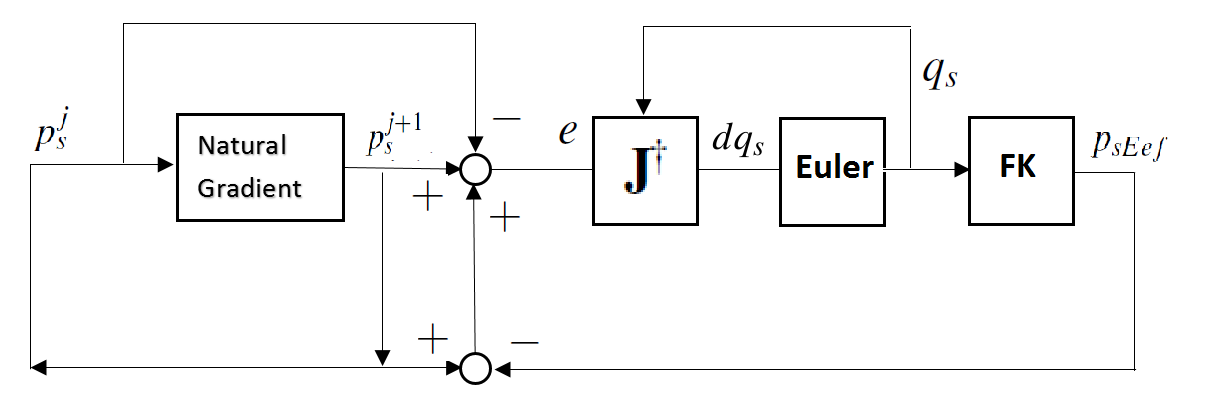
\includegraphics[scale=0.35]{figure/loopControl.png}
	\caption{Block diagram of the projection process}
	\label{loopControl}
\end{figure}
 \begin{figure}[h]
 	\centering
 	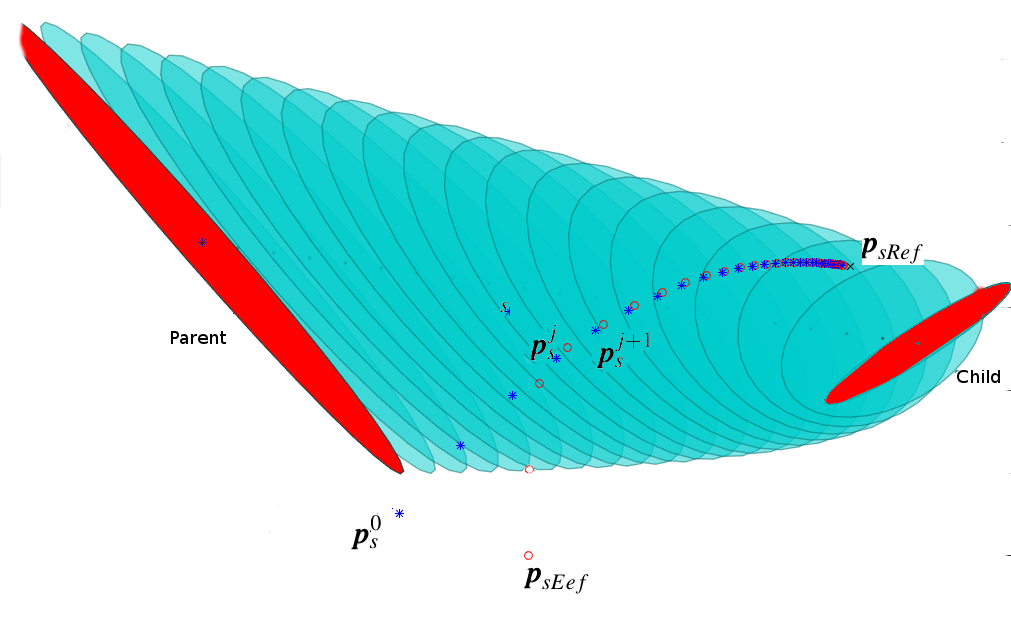
\includegraphics[scale=0.25]{figure/natProjFinal2.png}
 	\caption{Projection process of $\mb{p}_s^j$ onto $\mb{p}_{sRef}$with natural gradient descent guiding  $\mb{p}_{sEef}$, the pose of $\mb{q}_s$}
 	\label{ProjNat}
 \end{figure}
Despite being a bit slow due to all these projections, this way of solving the IK problem enables the algorithm to have different joints configuration for a same point and thus properly explore the C-Space while constraining the sample inside the Soft-Envelope.\\
Furthermore, to accelerate the process, we also exploit, during the projection, the series of intermediate created joints configuration $\mb{q}_s$ whose poses $\mb{p}_s^j$ are inside the Soft-Envelope to grow the RRT* tree (line 11-14).\\
{\fontfamily{qcr}\selectfont Get\_Membership\_SoftEnv($\mb{p}_s^j$)} evaluates which Gaussians of the Soft-Envelope is the closest to the pose $\mb{p}_s^j$ then if it belongs to it. It calculates the Mahalanobis distance from $\mb{p}_s^j$  to each of its $i^{th}$ Gaussian and then select the one with the smallest distance. Then this Gaussian, with its covariance matrix  $\mb{\Sigma}_{env}^{select}$ and center $\mb{\mu}_{env}^{select}$, is used to check if $\mb{p}_s^j$ is inside the Soft-Envelope with the Mahalanobis distance such that this condition $(\mb{p}_s^j-\mb{\mu}_{env}^{select})^{\trsp}(\mb{\Sigma}_{env}^{select})^{-1} ((\mb{p}_s^j-\mb{\mu}_{env}^{select})) < criteria$ holds. The value for the criteria is detailed in \cite{Filzmoser04amultivariate} (however, in practice, more strict values can be use). \\
In case we have a dimension reduction ($\alpha<100$), the Soft-Envelope is still used to find the gaussian with the smallest mahalanobis distance but its belonging is checked by using its corresponding Gaussian in the reduced Soft-Envelope.\\
\subsubsection{The core of PCT-RRT*}\leavevmode\par \label{CoreRRTStar} \label{coreRRTstarChapter}
While the work is more focused on the sampling in PCT-RRT*, the core of the algorithm, represented by the function {\fontfamily{qcr}\selectfont Extended\_RRTStar($G,\mb{q}_s,\mb{p}_s$)} in algorithm \ref{PCTCRRT} and whose process is illustrated in algorithm \ref{Extended_RRTStar}, remains almost the same as a RRT*.\\
\begin{algorithm}[H]
 \caption{PCT\_RRTStar($G$,$\mb{\Sigma}_{envSet}$,$\mb{\Sigma}_{redEnvSet}$,$\mb{\mu}_{envSet}$, $\alpha$)}\label{PCTCRRT}

\SetKwData{Left}{left}\SetKwData{This}{this}\SetKwData{Up}{up}
\SetKwFunction{Union}{Union}\SetKwFunction{FindCompress}{FindCompress}
\SetKwInOut{Input}{input}\SetKwInOut{Output}{output}

\setcounter{AlgoLine}{0}
\Input{In addition, $\mb{\Sigma}_p,\mb{\Sigma}_c,\mb{\mu}_p$ and $\mb{\mu}_c$ are assumed available for all the functions here}
\Output{Solution path connecting the parent and child gaussian}
\BlankLine
\textcolor{blue}{\emph{//First loop: creation of workspace and C-space samples,}\;}

	\While{TRUE or ALLOWED TIME}
	{
	\BlankLine
		$\mb{p}_{sRef} \leftarrow $ Sampling\_SoftEnv($\mb{\Sigma}_{envSet}, \mb{\Sigma}_{redEnvSet},\alpha$);
		
		$\mb{p}_{projRef} \leftarrow$	Axis\_SoftEnv\_Ortho\_Projection($\mb{p}_{sRef}$);
		
		$\mb{v}_{offset} = \mb{p}_{sRef}-\mb{p}_{projRef} $;
		\BlankLine
		$[\mb{\Sigma}_{sRef},flag_{sRef}]\leftarrow$\\ Get\_Membership\_SoftEnv($\mb{p}_{sRef},\mb{\Sigma}_{envSet}, \mb{\Sigma}_{redEnvSet}$,$\mb{\mu}_{envSet}$);
		\BlankLine
		
		$\mb{q}_s\leftarrow $Sampling\_CSpace\_0-2PI();
		
		$\mb{p}_s^j\leftarrow $ Forward\_Kin($\mb{q}_s$);
		
		$\mb{p}_{sEef}=\mb{p}_s^j$;
		\BlankLine
			
	\textcolor{blue}{\emph{//Second loop: Gradient projection and Tree growing}}
		\While{TRUE or ALLOWED TIME}
		{
			\BlankLine

			$[\mb{\Sigma}_2,flag2_{belong}]\leftarrow$\\ 
			Get\_Membership\_SoftEnv($\mb{p}_s^j,\mb{\Sigma}_{envSet}, \mb{\Sigma}_{redEnvSet}$,$\mb{\mu}_{envSet}$);
			\BlankLine
			
			\If{$flag2_{belong} == TRUE$}
			{
				
				$S_{path}\leftarrow $ Extended\_RRTStar($G,\mb{q}_s,\mb{p}_s$);
			}
			\BlankLine
				
			$\mb{p}_{proj} \leftarrow$	Axis\_SoftEnv\_Ortho\_Projection($\mb{p}_s^j$);
			
			$[\mb{\Sigma}_{g},\mb{\mu}_{g}] \leftarrow$ Gauss\_Lin\_Interpol($\mb{p}_{proj}$);
			
			$\mb{\mu}_{g} = \mb{\mu}_{g} + \mb{v}_{offset}$;
			\BlankLine
			\BlankLine
			$[\mb{p}_s^{j+1},flag_{diverge}] \leftarrow$\\
			 Natural\_Gradient($\mb{p}_s^{j},\mb{\Sigma}_{sRef},\mb{p}_{sRef},\mb{\Sigma}_{g},\mb{\mu}_{g}$);
			\BlankLine
			\If{$flag_{diverge} == TRUE$}
			{
			
				break;
			}
			
			$\mb{e}_1=\mb{p}_s^{j+1} - \mb{p}_s^{j}$;
			
			$\mb{e}_2=\mb{p}_s^{j+1} - \mb{p}_{sEef}$;
			
			$\mb{e}=\mb{e}_1+\mb{e}_2$;
			
			\BlankLine
			$\mb{J}\leftarrow$GetJacobian($\mb{q}_s$);
			
			$\mb{q}_s=\mb{q}_s+ \mb{J}^{\psin} \mb{e}$;
			
			$\mb{p}_{sEef}\leftarrow $ Forward\_Kin($\mb{q}_s$);
			
			\BlankLine
			$\mb{p}_s^{j} = \mb{p}_s^{j+1}$
			\BlankLine
			
			\If{$\mb{p}_s$ projected on $\mb{p}_{sRef}$}
			{
				$G \leftarrow $ Extended\_RRTStar($G,\mb{q}_s,\mb{p}_{sRef}$);
				
				break;
			}
		}
	}
\end{algorithm}

For the process of a conventional RRT*, new vertices and edges are added to $G=(Q_q,Q_p,E,Q_{sol})$ by growing the tree in the free C-space towards random selected states $\mb{q}_s$: for a new sample node $\mb{q}_s$ given to the RRT*, the nearest node from the $Q_q$ set is found in a euclidean distance metric. Then {\fontfamily{qcr}\selectfont Steer($\mb{q}_{Nearest},\mb{q}_s,\delta_r$) }  generates a new node $\mb{q}_{New}$ which is $\delta_r$ away from the nearest node $\mb{q}_{Nearest}$ towards the direction of the sample node $\mb{q}_s$. In case there is no collision in the line from the nearest node to the new created one, checked with the function {\fontfamily{qcr}\selectfont Collision\_Free($\mb{q}_{Nearest}, \mb{q}_{New}$) }, then a "choose parent" and "rewiring" steps are done for each new node such that it minimizes the cost of nearby nodes in the tree that are within a certain euclidean distance to the new node, found with  {\fontfamily{qcr}\selectfont Near($G,\mb{q}_{New}$) }.\\
The "choose parent" step evaluates the cost of each node in the neighborhood of $\mb{q}_{New}$ from the root node and select the one that minimizes this cost to be the parents of $\mb{q}_{New}$. The step of "rewiring" that follows evaluates each cost from $\mb{q}_{New}$  to its neighbor node, to which is added the cost from the root node of the tree to $\mb{q}_{New}$, in order to select the neighbor node that has the minimum cost such that $\mb{q}_{New}$ is its parent (or to be the children of $\mb{q}_{New}$ ). 
 {\fontfamily{qcr}\selectfont Cost($\mb{q}_{Near}$) } calculates the cumulative cost from the root node of the tree to $\mb{q}_{Near}$ and {\fontfamily{qcr}\selectfont CostIm($\mb{q}_{Near},\mb{q}_{New}$) } calculates the direct cost of going from $\mb{q}_{Near}$ to $\mb{q}_{New}$ (a more detailed explanation of the RRT* process is given in \cite{Karaman2011AnytimeMP} and \cite{KaramanRRTStar}).\\
 
 
In our variation of the RRT* (all changes are in red in algorithm \ref{Extended_RRTStar}), we use an additional set $Q_p$ which takes every pose found from forward kinematics of its corresponding joint configuration node added to $Q_q$. \\
An other change is made when the planner is looking for the nearest node to the sample one in {\fontfamily{qcr}\selectfont Nearest($G,\mb{q}_s,\mb{p}_s$)}. Instead of searching in C-space, it finds the closest node  $\mb{p}_{Nearest}$  in workspace from the $Q_p$ set to the sample pose $\mb{p}_s$ by using the Mahalanobis distance with the child covariance matrix $\mb{\Sigma}_c$. Since the two set $Q_q$ and $Q_p$ have the same number of node and are ordered in the same way, we also get $\mb{q}_{Nearest}$ which is used to grow the RRT* tree. While there is not concrete proof, we observed that this modification allows the tree to be more constrained around the Soft-Envelope. In fact, instead of having the nearest joint configuration to the  joint angles sample and thus growing a tree only based on joint angles without knowing anything about their poses, we decided to look for the nearest pose, which has more chance of being inside the Soft-Envelope  to grow the tree in C-space with its joint angles. A comparison can be found in figure \ref{Nearest} \\

\begin{figure}[h]
	\centering
	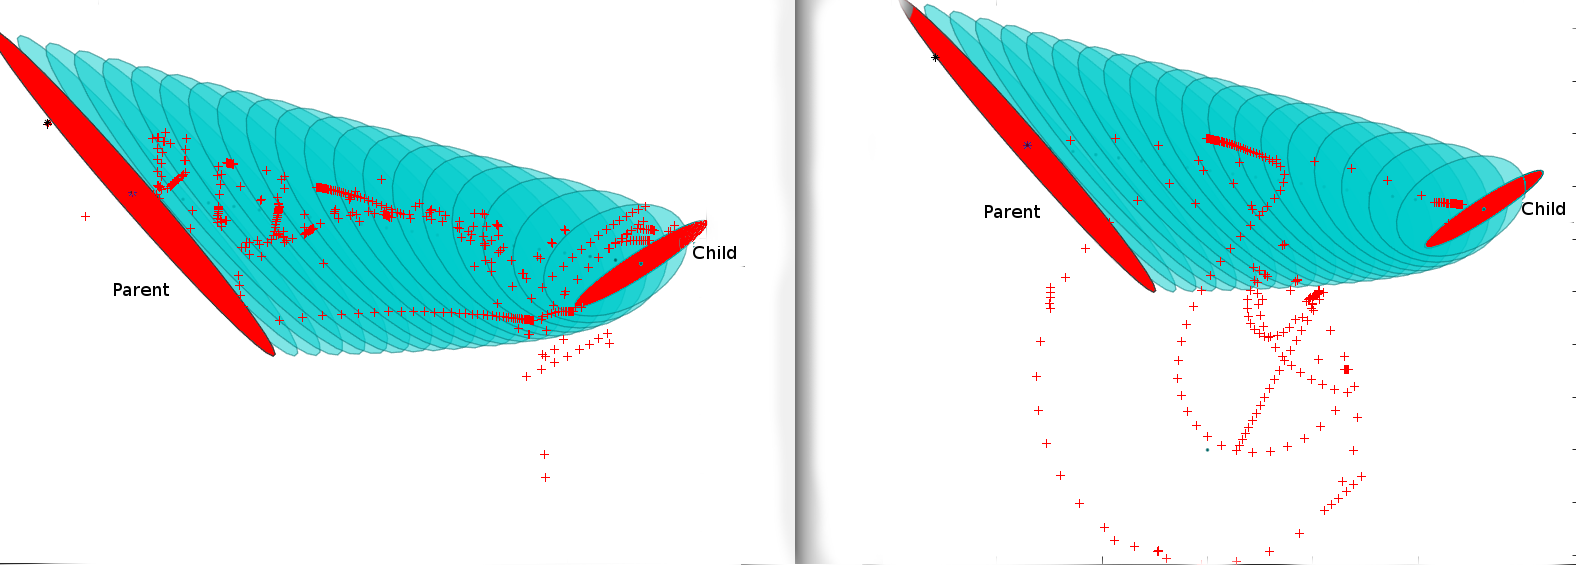
\includegraphics[scale=0.16]{figure/WithVsWithoutNearestChange.png}
	\caption{All poses in the tree (red cross) with the Nearest function look for: (left) nearest pose, (right) nearest joints angles; The left one is more constrained around the Soft-Envelope}
	\label{Nearest}
\end{figure}

We also changed the condition to tell when a path is found by the planner (line 22-27). When a new node $\mb{q}_{New}$ in C-space is added to the Tree, we use its corresponding pose $\mb{p}_{New}$ to calculate the Mahalanobis distance to the child Gaussian and evaluate its belonging with $(\mb{p}_{New}-\mb{\mu}_{c}^i)^{\trsp}(\mb{\Sigma}_{c})^{-1} ((\mb{p}_{New}-\mb{\mu}_{c}^i)) < criteria$ (value for $criteria$ mentioned in section \ref{PCT-RRT*}). If this condition holds, then a solution path from the parent to the child Gaussian  is found. We can then either directly update the next pair of parent/child Gaussian in order to plan for the next new local trajectory or continue the sampling to find a more optimal path until the allowed time is reached or any other criteria specified by the user is met. Local biasing can also be added to the sampling in algorithm \ref{SoftEnv_Sampling} once a path is found as suggested by Akgun \textit{and al.} in \cite{BarisRRT} in order to focus the sampling more around the best solution path to improve it faster . \\
 
 \begin{algorithm}[H]
  \caption{Extended\_RRTStar($G,\mb{q}_s,\mb{p}_s$)}\label{Extended_RRTStar}
 
 \SetKwData{Left}{left}\SetKwData{This}{this}\SetKwData{Up}{up}
 \SetKwFunction{Union}{Union}\SetKwFunction{FindCompress}{FindCompress}
 \SetKwInOut{Input}{input}\SetKwInOut{Output}{output}
 
 \setcounter{AlgoLine}{0}
 
 \Output{set of vertices and edges $G=(Q_q,Q_p,E,Q_{sol})$}
 \BlankLine
 
 \textcolor{red} {$[\mb{q}_{Nearest},\mb{p}_{Nearest}] \leftarrow$ Nearest($G,\mb{q}_s,\mb{p}_s$);}
 
 $\mb{q}_{New} \leftarrow$ Steer($\mb{q}_{Nearest},\mb{q}_s,\delta_r$);
 
 \If{Collision\_Free($\mb{q}_{Nearest}, \mb{q}_{New}$)}
 {
 	$Q_q \leftarrow Q_q \cup  \mb{q}_{New} $;
 	
 	$\mb{q}_{Min} \leftarrow  \mb{q}_{Nearest}$;
 	
 	$Q_{Near} \leftarrow$ Near($G,\mb{q}_{New}$);
 	
 	\ForAll{$\mb{q}_{Near} \in Q_{Near}$}
 	{
 		\If{Collision\_Free($\mb{q}_{Near}, \mb{q}_{New}$)}
 		{
 			\If{Cost($\mb{q}_{Near}$)+CostIm($\mb{q}_{Near},\mb{q}_{New}$)$<$Cost($\mb{q}_{New}$)}
 			{
 				$\mb{q}_{Min} \leftarrow Q_{Near}$;
 			}
 			
 		}
 	}
 	
 	$E \leftarrow E \cup (\mb{q}_{Min},\mb{q}_{New})$;
 	
 	\ForAll{$\mb{q}_{Near} \in Q_{Near}$\textbackslash $\mb{q}_{Min}$}
 	{
 		\If{Collision\_Free($\mb{q}_{Near}, \mb{q}_{New}$) and Cost($\mb{q}_{New}$)+CostIm($\mb{q}_{Near},\mb{q}_{New}$) $<$ Cost($\mb{q}_{Near}$)}
 		{
 			$\mb{q}_{Par} \leftarrow$ Parent($\mb{q}_{Near}$); 
 			
 			$E \leftarrow E$ \textbackslash $(\mb{q}_{Par},\mb{q}_{Near})$;
 			
 			$E \leftarrow E \cup (\mb{q}_{New},\mb{q}_{Near})$;
 		}
 	}
     
 
 \BlankLine
 	\textcolor{red} {$\mb{p}_{New}\leftarrow$ Forward\_Kin($\mb{q}_{New}$);}
 	
 	\textcolor{red} {	$Q_p \leftarrow Q_p \cup  \mb{p}_{New} $;}
 	
 	\textcolor{red}{ $dist\_goal \leftarrow$ MahalanobisDist($\mb{p}_{New},\mb{\Sigma}_{c},\mb{\mu}_{c}$);}
 	 
 	\textcolor{red} {\If{dist\_goal $<$ GaussBelongCrit}
 	{
 		$Q_{sol} \leftarrow Q_{sol} \cup {\mb{p}_{New}}$;
 	}
 	}
 }
 \end{algorithm}

\subsubsection{Sampling}\leavevmode\par \label{samplingSection}
The sampling that was done inside the Soft-Envelope follows the procedure illustrated by the pseudo-code in algorithm \ref{SoftEnv_Sampling}.
We use a goal biasing heuristic to either sample inside the child gaussian, which can drastically change the planning speed, or to uniformly sample inside the (reduced) Soft-Envelope (line 2-9). \\
When sampling inside the child Gaussian, the covariance matrix used to generate samples is just $\mb{\Sigma}_c$. Otherwise we sample uniformly inside the Soft-Envelope by first randomly selecting a pose, $\mb{p}_{sel}$,on the axis connecting the center of the parent and child Gaussians.\\
 {\fontfamily{qcr}\selectfont Gauss\_Lin\_Interpol($\mb{p}_{sel}$)} is then used with this pose to calculate the covariance matrix $\mb{\Sigma}_{sel}$ and center $\mb{\mu}_{sel}$ of the envelope Gaussian. To do so, this function performs the same linear interpolation of the covariance matrix as in equation \ref{equaInterCov} with  $\Delta d = \norm{\overrightarrow{\mb{\mu}_p\mb{\mu}_{sel}}}/{\norm{\overrightarrow{\mb{\mu}_p\mb{\mu}_c}}}$, and $\mb{\mu}_{sel} = \mb{p}_{sel}$. Limitations of the center $\mb{\mu}_{sel}$ calculation is also set by using the unit vector $\overrightarrow{\mb{U}_{\mb{\mu}_p\mb{\mu}_{c}}} = \overrightarrow{\mb{\mu}_p\mb{\mu}_{c}}/\norm{\overrightarrow{\mb{\mu}_p\mb{\mu}_{c}}}$: in case we have $\overrightarrow{\mb{U}_{\mb{\mu_{sel}}\mb{\mu_{c}}}} \neq \overrightarrow{\mb{U}_{\mb{\mu}_p\mb{\mu_{c}}}} $, then it means that the center $\mb{\mu}_{sel}$ is not in-between the two considered parent/child gaussians, ie it is outside from the perspective of the child gaussian, thus the covariance and center are set such as $\mb{\Sigma}_{sel}=\mb{\Sigma}_c$ and $\mb{\mu}_{sel}=\mb{\mu}_c$; in case of $\overrightarrow{U_{\mb{\mu}_{p}\mb{\mu}_{sel}}} \neq \overrightarrow{U_{\mb{\mu}_p\mb{\mu_{c}}}} $, then the center $\mu_{sel}$ is outside from the perspective of the parent gaussian, thus we have $\mb{\Sigma}_{sel}=\mb{\Sigma}_p$ and $\mb{\mu}_{sel}=\mb{\mu}_p$.\\
Once we have $\mb{\Sigma}_{sel}, \mb{\mu}_{sel}$, we then generate one sample from this gaussian with $\mb{\Sigma_{sel}}\mb{r}+\mb{\mu_{sel}}$, with $\mb{r} \in \mathbb{R}^{M \times 1}$ a vector with M random values. \\
In case a dimension reduction need to be perform ($\alpha<100$), we simply reduce the gaussian $\mb{\Sigma}_{sel}$ as explained in the section \ref{ReducedSoftEnvelope} with the algorithm \ref{AlgoRedSoftEnve} line (8-18) before using it to generate the sample. \\

\begin{algorithm}[H]
 \caption{Sampling\_SoftEnv($\mb{\Sigma}_{envSet}, \mb{\Sigma}_{redEnvSet},\alpha$)}\label{SoftEnv_Sampling}

\SetKwData{Left}{left}\SetKwData{This}{this}\SetKwData{Up}{up}
\SetKwFunction{Union}{Union}\SetKwFunction{FindCompress}{FindCompress}
\SetKwInOut{Input}{input}\SetKwInOut{Output}{output}

\setcounter{AlgoLine}{0}
\Input{In addition, $\mb{\Sigma}_p,\mb{\Sigma}_c,\mb{\mu}_p$ and $\mb{\mu}_c$ are assumed available for all the functions here}
\Output{Sample $\mb{q}_s$ in C-space }
\BlankLine
 $randProb \leftarrow $Random\_Real\_From0To2PI();
 
	\uIf{randProb $<$ GoalBias}
	{
		$\mb{\Sigma}_{sel} = \mb{\Sigma}_c$;
	}
	\Else
	{
	 	$randNum \leftarrow $Random\_Real\_From0To2PI();
	 	
	 	$\mb{U}_{axis}=(\mb{\mu}_c - \mb{\mu}_p)/\overrightarrow{{\mb{\mu}_p\mb{\mu}_{c}}}$;
	 	
	 	$\mb{p}_{sel}=\mb{\mu}_p+\mb{U}_{axis}*(randNum \times \overrightarrow{{\mb{\mu}_p\mb{\mu}_{c}}})$;
	 	
	 	$[\mb{\Sigma}_{sel},\mb{\mu}_{sel}] \leftarrow$ Gauss\_Lin\_Interpol($\mb{p}_{sel}$);
	}
	\uIf{$\alpha$ $<$ 100}
	{
		$\mb{\Sigma}_{redSel} \leftarrow $ reduction $\mb{\Sigma}_{sel}$ as in algorithm \ref{MixSoftEnvelope} (line 8-18);
		
		$\mb{q}_s \leftarrow $ Sample\_Gaussian($\mb{\Sigma}_{redSel}$);
	}
	\Else
	{
		$\mb{q}_s \leftarrow $ Sample\_Gaussian($\mb{\Sigma}_{sel}$);
	}
\end{algorithm}

\subsubsection{Projection - Natural gradient descent}\leavevmode\par

Because we are using a Mahalanobis distance w.r.t to the Gaussians of the Soft-Envelope instead of an euclidean distance to update the pose $\mb{p}_s^j$ for the projection, the natural gradient descent is chosen \cite{WhyAdaptiveGrad} to minimize the projection cost. The cost of the gradient takes into account two influences: the Gaussian that the reference pose $\mb{p}_{sRef}$ belongs to (that we are calling goal Gaussian in this subsection) and the Soft-Envelope itself. While using only the goal gaussian is possible for the projection, integrating the influence of the Soft-Envelope makes the valley of the gradient cost function bend more toward it. In other words, the line created by the projected points is a little bit more curved towards the Soft-Envelope. This behavior is desirable to speed the growth of the Tree since every joint configuration whose pose is inside the envelope is used to grow the RRT* tree (algorithm \ref{PCTCRRT} line 12-14).\\
The goal gaussian is determined with the function {\fontfamily{qcr}\selectfont Get\_Membership\_SoftEnv($\mb{p}_{sRef}$)} which output the covariance matrix $\mb{\Sigma}_{sRef}$ of the goal gaussian with $\mb{p}_{sRef}$, used as the center of the goal gaussian (algorithm \ref{PCTCRRT} line 6).\\
The influence of the Soft-Envelope is taken into account by first projecting the pose $\mb{p}_s^j$ onto the axis created by the center $\mb{\mu}_p, \mb{\mu}_c$ of the parent/child gaussians with the function {\fontfamily{qcr}\selectfont Axis\_SoftEnv\_Ortho\_Projection($\mb{p}_s^j$)} that uses the formula $\mb{p}_{proj} = \mb{\mu}_p + \mb{p}_{tmpProj}$ with $\mb{p}_{tmpProj}=\frac{ (\overrightarrow{\mb{\mu}_p\mb{p}_s^j} \cdot \overrightarrow{\mb{\mu}_p\mb{\mu}_c})}{\norm{\overrightarrow{\mb{\mu}_p\mb{\mu}_c}}^2}\overrightarrow{\mb{\mu}_p\mb{\mu}_c} $ \\
The projected point $\mb{p}_{proj}$ on the axis is then used in the function {\fontfamily{qcr}\selectfont Gauss\_Lin\_Interpol($\mb{p}_{proj}$)} to find the center $\mb{\mu}_g^j$ and covariance $\mb{\Sigma}_g^j$ of the gaussian inside the Soft-Envelope that influences the gradient cost function (algorithm \ref{PCTCRRT} line 15-16).\\

One has to notice that $\mb{p}_{sRef}$ which is not necessarily on the axis of the parent-child center was chosen as the center for $\mb{\Sigma}_{sRef}$. The consequence is that it creates an offset in the natural gradient projection of $\mb{p}_s^j$ onto $\mb{p}_{sRef}$  . In order to correct it, the same orthogonal projection function {\fontfamily{qcr}\selectfont Axis\_SoftEnv\_Ortho\_Projection($\mb{p}_{sRef}$)} is used on the reference sample $\mb{p}_{sRef}$ to calculate the "offset" $\mb{v}_{offset}$ which will be added to the center $\mb{\mu}_g^j$ before being used in the natural gradient update (algorithm \ref{PCTCRRT} line 4-5 and 17).\\

The natural gradient is calculated by using the Mahalanobis metric such as: 
\begin{equation}
			 coeff = \frac{\norm{\overrightarrow{\mb{\mu}_c\mb{\mu}_p}}}{(\mb{\mu}_p-\mb{\mu}_c)^{\trsp}\mb{\Sigma}_c^{-1}(\mb{\mu}_p-\mb{\mu}_c)}
\end{equation}
\begin{subnumcases}{}
			 F_{Goal}=(\mb{p}_s^j - \mb{p}_{sRef})^{\trsp}\mb{\Sigma}_{sRef}^{-1}(\mb{p}_s^j - \mb{p}_{sRef}) \\
			 F_{Env}=(\mb{p}_s^j - \mb{p}_{proj}^j)^{\trsp}\mb{\Sigma}_{g}^{-1}(\mb{p}_s^j - \mb{p}_{proj}^j)
\end{subnumcases}
\begin{subnumcases}{}
 			\mb{dF}_{Goal}=2\mb{\Sigma}_{sRef}^{-1}(\mb{p}_s^j - \mb{p}_{sRef}) \\
			\mb{dF}_{Env}=2\mb{\Sigma}_{g}^{-1}(\mb{p}_s^j - \mb{p}_{proj}^j)
\end{subnumcases}
The update of $p_s^j$ is done with :
\begin{equation}
	\mb{p}_s^j = \mb{p}_s^j+\delta_{n}(\mb{\Sigma}_{g}(-coeff \times \mb{dF}_{Env} )+\mb{\Sigma}_{sRef}(-coeff \times \mb{dF}_{Goal} ))
	\label{equCostNatGrad}
\end{equation}

with $\delta_{n}$ the natural gradient stepsize. \\
The choice of the stepsize is important for a correct convergence of the projection. Numerous techniques exist to calculate the stepsize of a gradient descent projection, but most of them still create too much points because of the value of the stepsize which is often chosen small to avoid divergence. In addition of being slow, the number of projected points can also be too dense, which might create an unwanted biasing of the tree growth toward some specific regions other than the child gaussian.\\
Since the goal $\mb{p}_{sRef}$ of the natural gradient projection is different at new each iteration, we use an adaptive step-size for each new projection by using the same formula illustrated in \cite{AdaptiveStepSizeNatGrad} used in a reinforcement learning framework, p. 289 equation 6. 

\begin{subnumcases}{}
	step1 = (coeff \times \mb{dF}_{Goal})^{\trsp} \mb{\Sigma}_{sRef} (coeff \times \mb{dF}_{Goal}) \\
	step2 =	(coeff \times \mb{dF}_{Env})^{\trsp} \mb{\Sigma}_{g} (coeff \times \mb{dF}_{Env}) \\
	\delta_{n} = \frac{1}{\sqrt{(step1+step2)}}
	\label{stepSizeAdaptive}
\end{subnumcases}

The calculation of $\delta_{n}$ is only done once at the beginning of each new projection (ie for each new sample $\mb{p}_{sRef}$), which allows a faster projection as the calculated poses at the beginning are more distant. In fact, if the first next pose updated by the natural gradient converges towards $\mb{p}_{sRef}$, then the rest of the projection will also converge for the same step-size because the Mahalanobis distance from each new updated pose to  $\mb{p}_{sRef}$ with $\mb{\Sigma}_{sRef}$ is decreasing.\\
Since the context of application of this formula is different, we implement an additional step to avoid divergence of the projection. If the Mahalanobis distance using the first updated pose $\mb{p}_s^{j+1}$ to $\mb{p}_{sRef}$ with $\mb{\Sigma}_{sRef}$ is bigger than the Mahalanobis distance using the original pose sample $\mb{p}_s^{j}$, then it means that the step of the new updated pose was too big and then the projection will diverge. We corrected this problem by diminishing the step-size for N iterations until convergence ( $\delta_{n}= \delta_{n} \times a$ with $0<a<1$, in a similar way as the step-size line search backtracking method), with N a parameter defined by the user. If after N iterations, the criteria is still not met, then the projection is not evaluated (algorithm \ref{PCTCRRT} line 19-21).\\
A comparison with a projection using a stepsize found with backtracking line search is pictured in figure \ref{Stepsize}

\begin{figure}[h]
	\centering
	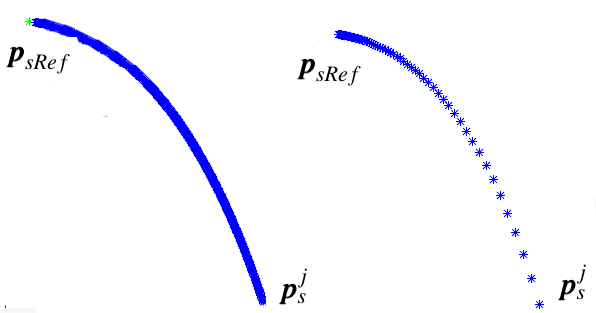
\includegraphics[scale=0.3]{figure/stepSizeComparison.png}
	\caption{Natural gradient projection of $\mb{p}_s^j$ onto $\mb{p}_{sRef}$ with: (left) stepsize found with backtracking line search method, (right) our stepsize}
	\label{Stepsize}
\end{figure}

\section{Experiments and results}
  In this section, our objectives is to show firstly if our method can successfully be used to accomplish the task and secondly to uncover how our algorithm influences, with and without dimension reduction, the generation of an end-to-end trajectory w.r.t the intention of the user. As we assimilated his intention when demonstrating the skill to the biggest variance of the Gaussians in the model, we are interested to see how the end-effector moves accordingly and w.r.t the Soft-Envelope in order to avoid an obstacle. For this purpose, we tested our method with two different tasks with different models. 
  Using these two tasks, the performance of our method is assessed and its runtime is also compared with the RRT-JT introduced by Vandeweghe \textit{et al.} in \cite{Vandeweghe_2007_5981}, a planner renowned to be fast in the sampling-based planning literature. It uses the Jacobian transform to bias the growth of the tree toward a pose while exploring the C-space. For our experiment, we have made 3 modifications to adapt our problem in Lfd: the goal sample comes from the sampling inside the child Gaussian, the search for the nearest node when it is biased towards the goal sample and the criteria to end the planning are changed according to our method explained in section \ref{CoreRRTStar}. Otherwise the algorithm is the same as described in his paper (and thus does not used any constrained area like the Soft-Envelope). \\
  
For the experiment, we first used kinesthetic teaching with a real 6-dof Kinova Jaco arm mounted on a robot platform (figure \ref{Pic_kinesthetik_teaching}) to collect keyframes data and a simulated robot in simulation to emulate its behavior and obtain results.\\
We then evaluated our algorithm with Moveit-Rviz simulator. The program is used as an input for our algorithm written in C++. The behavior of the robot arm was tested with 2 different tasks. The setup for each of them was with a 0.61m x 1.22m x 0.73m table on which were disposed different objects from the YCB. Simulation was done on a Lenovo computer with  a Intel Core i7-5600U CPU 2.60GHz × 4 processor and Nvidia GeForce 940M graphic card.\\
We tested our algorithm with 2 simple tasks whose skill models, learned with 7 successful demonstrations, are only encoded with two Gaussians. In the next figures, the parent Gaussian is in red and the child one is in blue. For each task, the algorithm was run 7 times, with dimension reduction of $\alpha = 85 \%$ and without it. Moreover, the initial configuration of the arm is placed above the table with its end-effector inside the red Gaussian. \\

\subsection{Task 1: Pick and drop}
\begin{figure}[h]
	\centering
	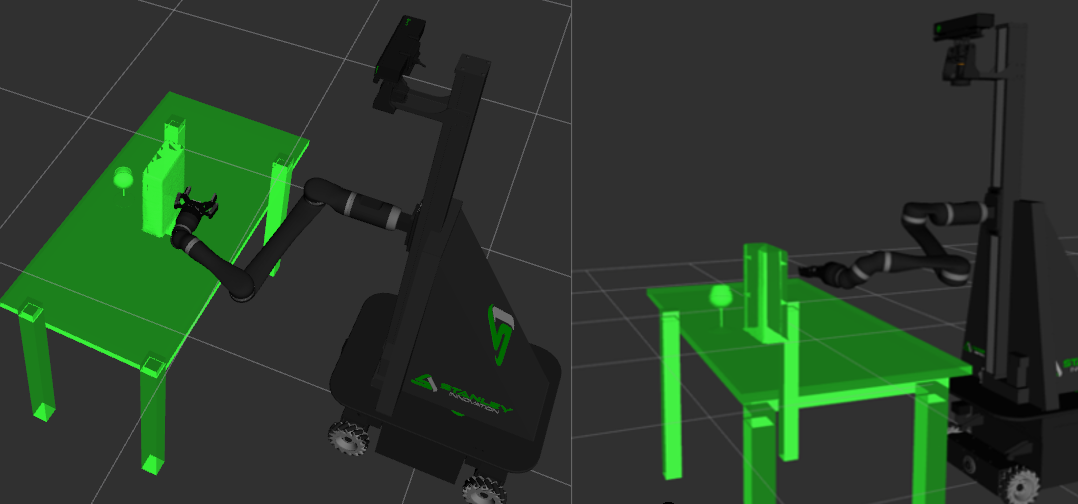
\includegraphics[scale=0.22]{figure/task1Scenario.png}
	\caption{Setup of the task 1: a plastic wine glass and a Cheez-it box on the table}
	\label{task1Scenario}
\end{figure}
The task is to have the end-effector, that is holding a small object(cherry fruit), goes above a wine glass in front of it and release its gripper to drop the object inside. During the execution, the Cheez-It box is used to obstruct the arm movement as shown in figure \ref{task1Scenario}. \\
The skill of the model is represented with the Gaussians in figure \ref{trajectoriesTask1}. We intentionally demonstrated it such that the robot has more freedom/variance along the long side of the table at its initial configuration (as shown with the variance of the red Gaussian). In the logic that the end-effector can release the object it is holding  in a relative distance above the glass and still accomplish the task (as long as the object end up inside the glass), we show more variance in the vertical direction w.r.t to the glass/table (blue gaussian).
In this task, our objective is to show how our algorithm with dimension reduction influences the trajectory generation toward directions reflected by the variances of the Gaussians in the model, even though their variance are already clearly defined . Results of the generated trajectories are pictured in figure \ref{trajectoriesTask1} \\
\begin{figure}[h]
	\centering
	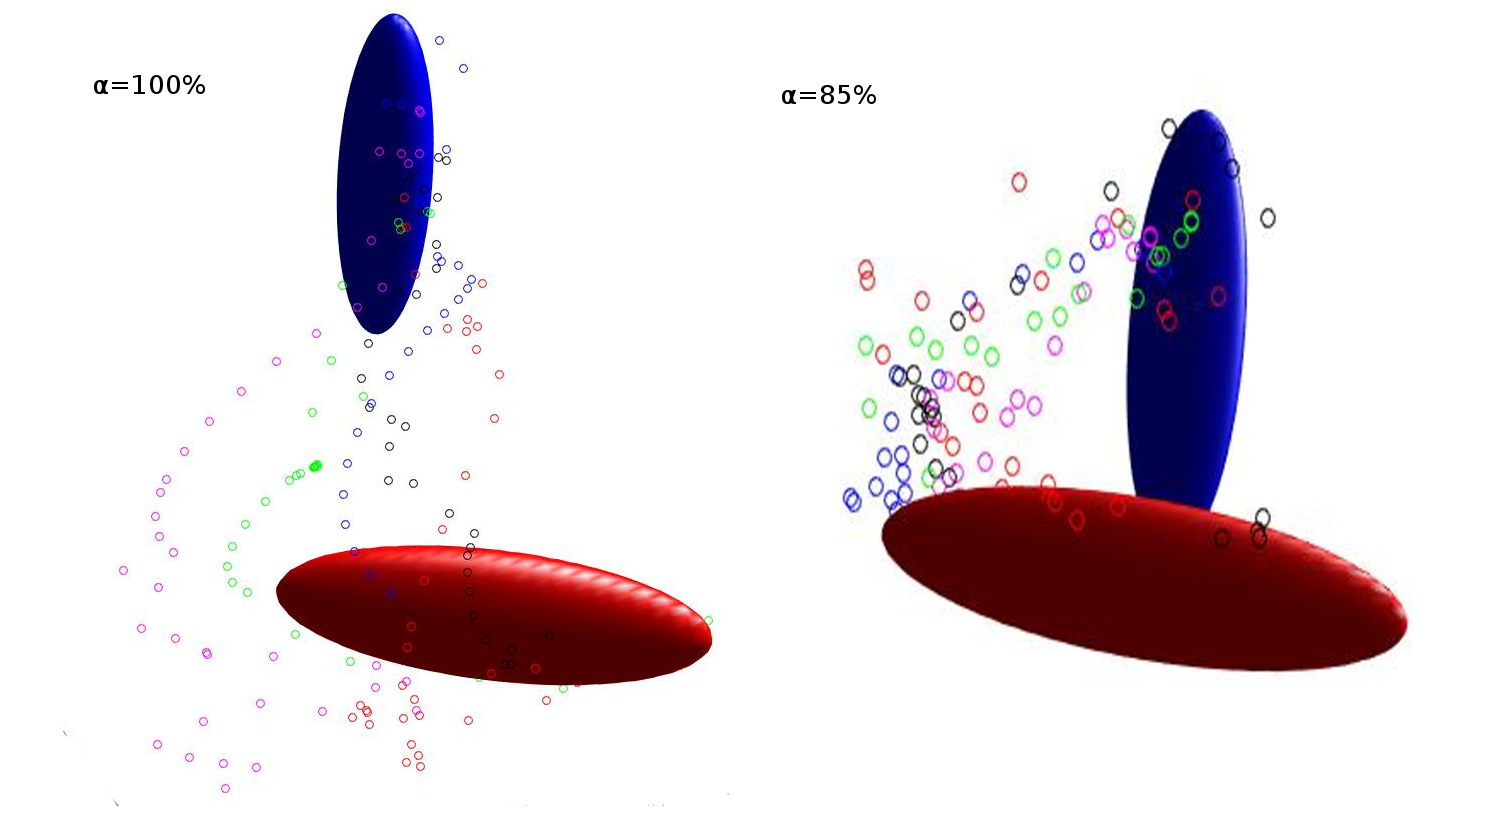
\includegraphics[scale=0.16]{figure/plotMixedTask1.png}
	\caption{Plot of 5 different trajectories (distinction by color) in x,y,z space for task 1 with (right image) $\alpha = 85\%$ and (left image)$\alpha = 100\%$ }
	\label{trajectoriesTask1}
\end{figure}
We can clearly see that all the trajectories with dimension reduction first follow the variance of the first gaussian (avoiding the obstacle by its side) before going up (certainly following the variance of the second one), which shows the influence of our algorithm. While the trajectories don't look as optimal as the one calculated without reduction, they are more coherent w.r.t the demonstration given by the user (and in addition, given the same situation (example of pouring water into a glass), most people probably would have avoided the large obstacle the same way). \\
\subsection{Task 2: Pick and place}
\begin{figure}[h]
	\centering
	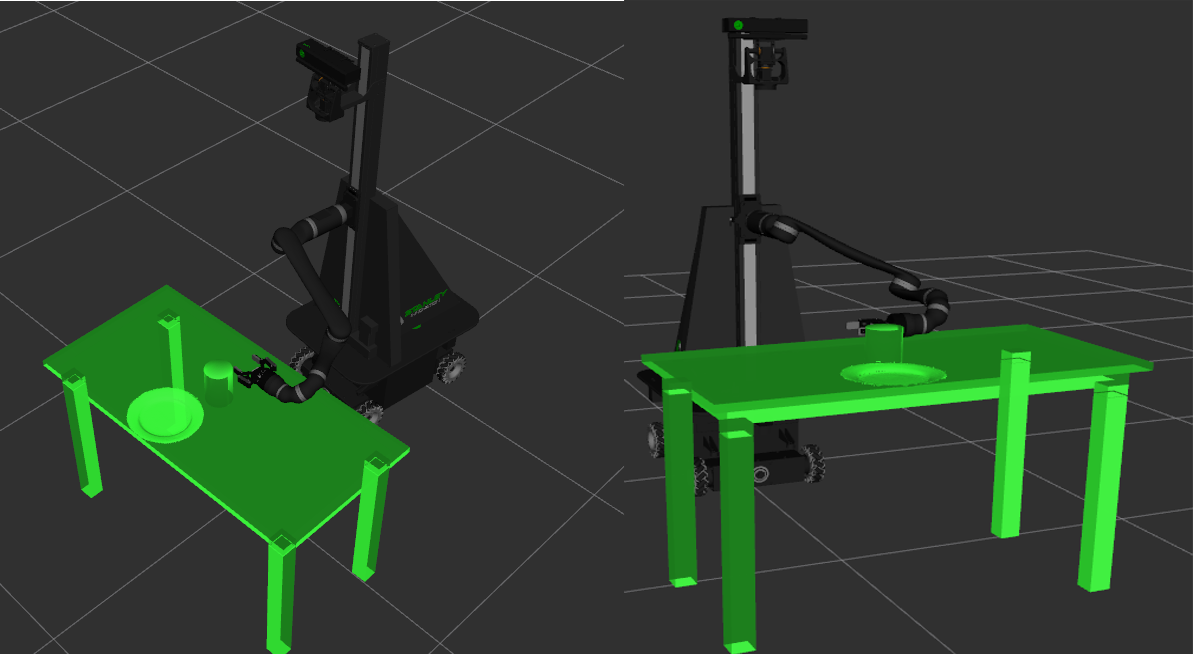
\includegraphics[scale=0.2]{figure/task2Scenario.png}
	\caption{Setup of task 2: a plate and a coffee can on the table}
	\label{task2Scenario}
\end{figure}
The setup in task 2 is pictured in figure \ref{task2Scenario} in which we used the coffee can in the middle to hinder the motion. The task is to have the end-effector pick an object on the table (a fruit for instance) and place it on a plate in front of it. \\
 For the demonstration, we wanted the end-effector to always begin at the same position above the table but with little more variance in the vertical direction w.r.t the table (red Gaussians). Then, when proceeding to deposit the object on the plate, it can cover it entire space and also release the object at certain height, which is why the blue Gaussians is spherical/ellipsoidal.\\
The objective in this task is to show how, with less obvious variance from the Gaussians (unlike the task 1), our algorithm encapsulates and uses their principal direction to influence the creation of trajectories.\\
We can clearly see that without dimension reduction, the trajectories are more messy, in particular the blue and black one who are starting going left but completely deviated to the right. Furthermore, one small detail to be noticed about the influence of our algorithm with dimension reduction: trajectories start more by going along the principal component of the first gaussian unlike the other case. 

\begin{figure}[h]
	\centering
	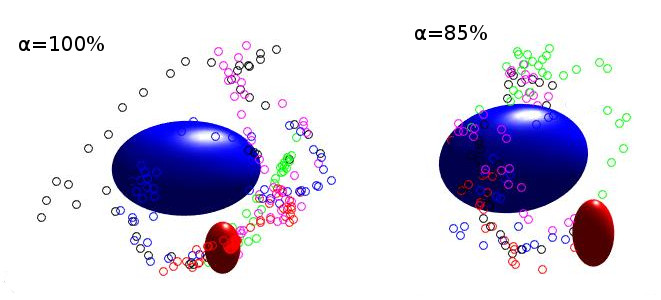
\includegraphics[scale=0.38]{figure/gaussianTask2.jpg}
	\caption{Plot of 5 different trajectories (distinction by color) in x,y,z space for task 2 with (right image) $\alpha = 85\%$ and (left image)$\alpha = 100\%$ }
	\label{task2ModelGaussian}
\end{figure}
\subsection{Tasks Performance}
\begin{figure}[h]
	\centering
	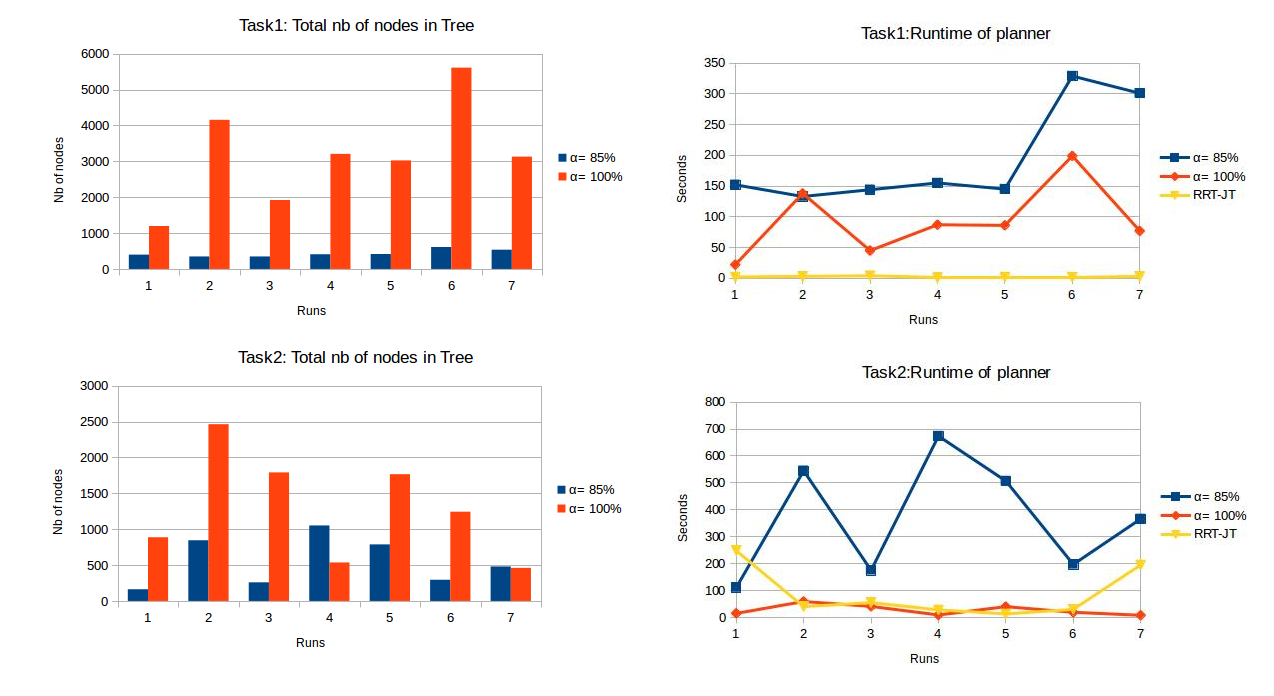
\includegraphics[scale=0.27]{figure/RunTimeAndNbNodeTask1_2.png}
	\caption{Plots: total number of node in tree (col. 1) and Runtime(col. 2) for the first (row 1) and second (row 2) task }
	\label{plotGraphAll}
\end{figure}
All the trajectory displayed in the previous subsections were able to successfully  perform the task, however the performances with and without dimension reduction are different, as shown with the runtime and total number of node in the tree in the figure \ref{plotGraphAll} for the first and second task. \\

As expected, both tasks display similar performance results: it takes less time without dimension reduction because more joints configuration node, whose poses are inside the full Soft-Envelope, are used to grow the tree than with the reduced Soft-Envelope. Indeed, since the Gaussians of the Soft-Envelope are reduced and thus their size is smaller, the poses from the natural gradient projection belongs more easily to the full Soft-Envelope than to the reduced one, which is why the total number of nodes in the tree is in general bigger than the one with reduce dimension.\\

In addition, we also compare the speed performance of our method with the RRT-JT planner, known to be fast thanks to its biasing in workspace using the Jacobian transform. We can clearly see that it outperforms our algorithm with and without dimension reduction for the first task but holds similar performance or is even outperformed by our method without dimension reduction in the second task.\\
The reason for such fast planning for the first task is because of the variance of the child Gaussian (blue one) which is large in the vertical direction. Hence, using the Jacobian biasing method with the (goal) samples from this Gaussian is effective because it does not run into the Cheez-it box obstacle. In the case of our algorithm, it is slower because of all the projections for each sample inside the Soft-Envelope: even if more nodes are used to grow our tree for one sample inside the Soft-Envelope (used of intermediate projected joints angles whose poses are inside the Soft-Envelope to also grow the tree), they may not all lead the tree to converge towards the child Gaussian.\\
For the second task, RRT-JT is, for some runs, outperformed by our method because even if the goal samples from the child (blue) Gaussian cover some large space above the table, it is sometimes not enough. In fact, the biasing of the tree to these goal samples with the Jacobian transform makes the tree go straight into the obstacle. It is however still able to complete the goal thanks to its alternation from its biasing feature to a simple, complete RRT. In addition, there were few trials that we did not illustrated in the result graph because even after waiting for more than 5-6 minutes, the RRT-JT planner was still not able to find any solutions.\\
 Even though this could also have occur with the first task, the difference is, in addition of the difference of child Gaussian variance, the position of the obstacle that is closer to the end-effector than the task 1, making the tree runs more into the obstacle when biasing it the Jacobian transform. With our method, the planner is able to quickly find a path thanks to the Soft-Envelope which indicates a way to quickly bypass the too close obstacle.

\section{Discussion}
In general, our planner is not design to be fast, but depending on the scenario it can hold good performance as in task 2. However it introduces a rather a new approach, to the best of the author's knowledge, that is easily adapted to Learning from demonstration work with the skill encoded with multivariate Gaussians, to constrain an area in workspace, focus the search around it and toward one direction related to user intention and plan accordingly. 
Moreover, if speed is a concern, our method can easily be combine with Jacobian transform from the RRT-JT to benefit from its biasing features.\\
Although we have mentioned 
\section{Future Work}
In this work, we have presented an approach that depends on the skill model to generate trajectory with sampling-based planner, and can further influence the planning by indicating one direction in to avoid obstacles. However, the model may not be fully representative of the direction to take in order to avoid obstacles depending on their form. The logical next step would be to integrate the environment, encapsulate the shapes and variances of the objects with a kinect for instance, with the variance of the model to calculate more precisely the best direction to take in order to avoid obstacles.
An other direction of work could be to further improve the algorithm such that it could plan a trajectory with dynamic obstacles (one direction of work is to use the RRTx suggested by Otte \textit{et al.} in \cite{RRTx}). 

\section{Conclusion}
We have presented a trajectory planner combined with a learned skill from keyframes demonstration. The concept of Soft-Envelope was proposed to constrain the area between two keyframes gaussians in which an extension of the RRT*, PCT-RRT*, was used to find a non-collision and available configuration space path linking two considered gaussians whose correspondent poses were around/inside the Soft-Envelope. The planner interleaves the exploration of C-space while being constrained in an area in workspace by using a double sampling process combined with gradient projection and jacobian.
The algorithm was successfully tested with two different tasks in simulation, showing the possible influences of the model on the motion of the end-effector.

\section{Acknowledgements}
The author would like to thank Aude Billard for making this joint research possible, Andrea L. Thomaz and Akgun Baris for the valuable time that they spent for help and discussions.
%%%%%%%%%%%%%%%%%%%%%%%%%%%%%%%%%%%%%%%%%%%%%%%%%%%%%%%%%%%%%%%%%%%%%%%%%%%%%%%%

\bibliography{bible}


\end{document}
